% mnras_template.tex
%
% LaTeX template for creating an MNRAS paper
%
% v3.0 released 14 May 2015
% (version numbers match those of mnras.cls)
%
% Copyright (C) Royal Astronomical Society 2015
% Authors:
% Keith T. Smith (Royal Astronomical Society)

% Change log
%
% v3.0 May 2015
%    Renamed to match the new package name
%    Version number matches mnras.cls
%    A few minor tweaks to wording
% v1.0 September 2013
%    Beta testing only - never publicly released
%    First version: a simple (ish) template for creating an MNRAS paper

%%%%%%%%%%%%%%%%%%%%%%%%%%%%%%%%%%%%%%%%%%%%%%%%%%
% Basic setup. Most papers should leave these options alone.
\documentclass[a4paper,fleqn,usenatbib]{mnras}

% MNRAS is set in Times font. If you don't have this installed (most LaTeX
% installations will be fine) or prefer the old Computer Modern fonts, comment
% out the following line
\usepackage{newtxtext,newtxmath}
% Depending on your LaTeX fonts installation, you might get better results with one of these:
%\usepackage{mathptmx}
%\usepackage{txfonts}

% Use vector fonts, so it zooms properly in on-screen viewing software
% Don't change these lines unless you know what you are doing
\usepackage[T1]{fontenc}
\usepackage{ae,aecompl}

%%%%% AUTHORS - PLACE YOUR OWN PACKAGES HERE %%%%%

% Only include extra packages if you really need them. Common packages are:
\usepackage[dvipdfmx]{graphicx}	% Including figure files
\usepackage{amsmath}	% Advanced maths commands
\usepackage{amssymb}	% Extra maths symbols
\usepackage{multicol}
\usepackage{siunitx}
\usepackage{bmpsize}
\usepackage[anythingbreaks]{breakurl}

\def\startdata{\if@table@not@headed\kill\caption{\\%
    \@tablecaption}\endhead\hline\endfoot%
  \fi%
}

\def\enddata{% 
 \crcr 
 \noalign{\vskip .7ex}% 
 \before@enddata 
 \endtabular 
 \setbox\pt@box\lastbox 
 \pt@width\wd\pt@box\box\pt@box 
}% 


\newcommand{\aprx}{\raise.17ex\hbox{$\scriptstyle\sim$}}

%%%%%%%%%%%%%%%%%%%%%%%%%%%%%%%%%%%%%%%%%%%%%%%%%%

%%%%% AUTHORS - PLACE YOUR OWN COMMANDS HERE %%%%%

% Please keep new commands to a minimum, and use \newcommand not \def to avoid
% overwriting existing commands. Example:
%\newcommand{\pcm}{\,cm$^{-2}$}	% per cm-squared

%%%%%%%%%%%%%%%%%%%%%%%%%%%%%%%%%%%%%%%%%%%%%%%%%%

%%%%%%%%%%%%%%%%%%% TITLE PAGE %%%%%%%%%%%%%%%%%%%

% Title of the paper, and the short title which is used in the headers.
% Keep the title short and informative.
\title[SPIDERMAN]{SPIDERMAN}

% The list of authors, and the short list which is used in the headers.
% If you need two or more lines of authors, add an extra line using \newauthor
\author[T. Louden, L. Kreidberg]{Tom Louden$^{1}$\thanks{E-mail: t.m.louden@warwick.ac.uk} and Laura Kreidberg$^{2}$\\
$^{1}$Department of Physics, University of Warwick, Coventry, CV4 7AL, UK\\
$^{2}$Department of Physics, University of America, America, America, America}

% These dates will be filled out by the publisher
\date{Accepted XXX. Received YYY; in original form ZZZ}

% Enter the current year, for the copyright statements etc.
\pubyear{2015}

% Don't change these lines
\begin{document}
\label{firstpage}
\pagerange{\pageref{firstpage}--\pageref{lastpage}}
\maketitle

% Abstract of the paper
\begin{abstract}

\end{abstract}

% Select between one and six entries from the list of approved keywords.
% Don't make up new ones.
\begin{keywords}
planets and satellites: individual (WASP 52b)---stars: individual (WASP 52)---techniques: spectroscopic---planets and satellites: atmospheres---celestial mechanics---atmospheric effects
\end{keywords}

%%%%%%%%%%%%%%%%%%%%%%%%%%%%%%%%%%%%%%%%%%%%%%%%%%

%%%%%%%%%%%%%%%%% BODY OF PAPER %%%%%%%%%%%%%%%%%%

\section{Introduction}\label{sec:introduction}

BATMAN \citep{Kreidberg2015a}

\section{Observations}\label{sec:Observations}

\section{Method}\label{sec:method}

\begin{figure}
\begin{center}
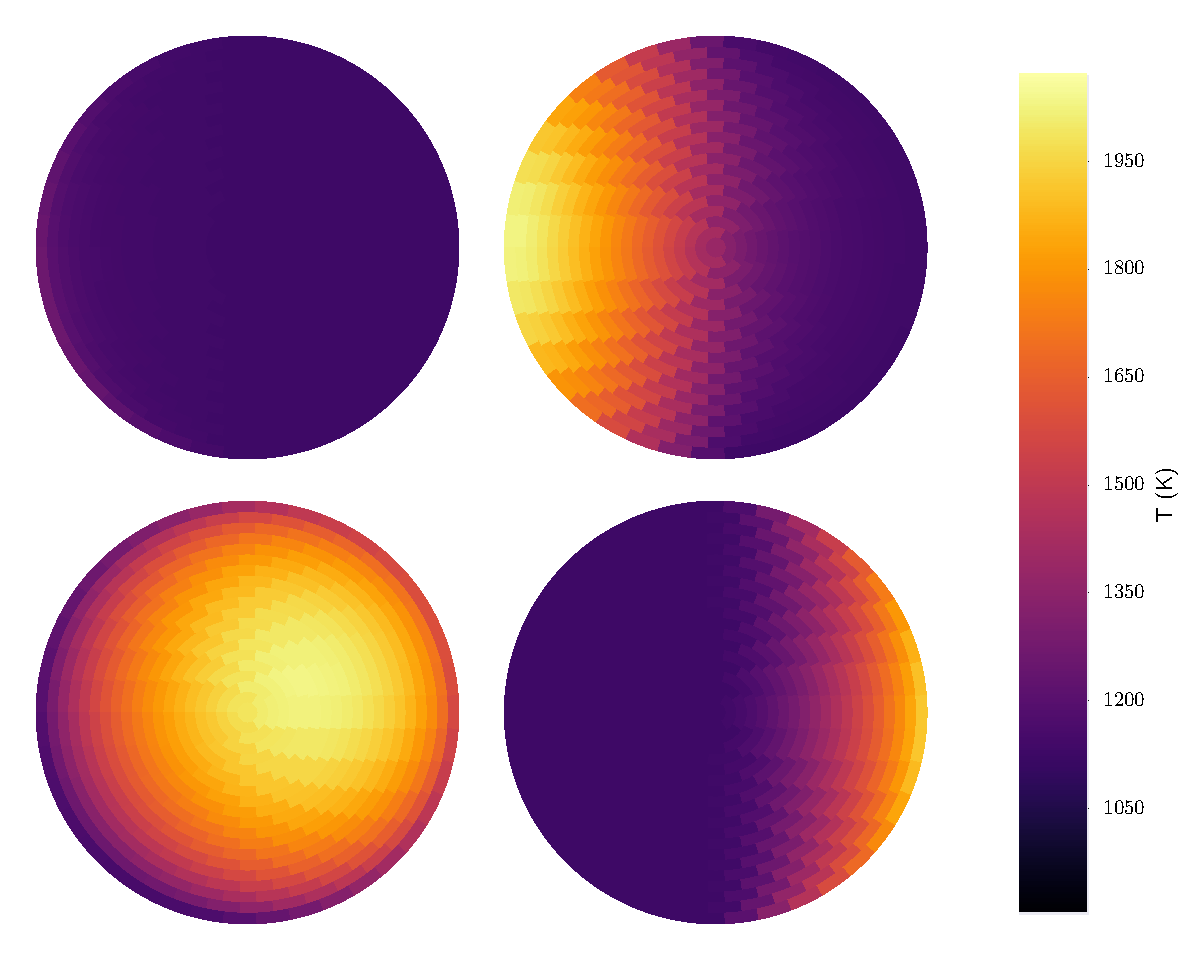
\includegraphics[width=\columnwidth]{img/b53.pdf}
\caption{This is a caption}
\label{fig:extract_region}
\end{center}
\end{figure}

\subsection{Fitting procedure}\label{sec:fitting}

\section{Results}\label{sec:results}

\subsection{transmission spectra}

\subsection{Updated system parameters}\label{sec:system}

\section{Discussion}\label{sec:Discussion}

\subsection{Spot crossing event}\label{sec:spotcross}

\section{Conclusions}

\section*{Acknowledgements}

The majority of this work was carried out at the kavli summer program in physics 2016. T.L extends his gratitude to the program organisers, in particular Jonothan Fortney and Pascale Geurard.

T.L. is supported by a STFC studentship. P.W. is supported by a STFC consolidated grant (ST/L000733/1).

%%%%%%%%%%%%%%%%%%%%%%%%%%%%%%%%%%%%%%%%%%%%%%%%%%

%%%%%%%%%%%%%%%%%%%% REFERENCES %%%%%%%%%%%%%%%%%%

% The best way to enter references is to use BibTeX:

\bibliographystyle{mnras}
%\bibliography{/home/astro/phrmat/Documents/BibTeX/Papers-LowEUV}
\bibliography{bibliography}
%\bibliography{example} % if your bibtex file is called example.bib


% Alternatively you could enter them by hand, like this:
% This method is tedious and prone to error if you have lots of references
%\begin{thebibliography}{99}
%\bibitem[\protect\citeauthoryear{Author}{2012}]{Author2012}
%Author A.~N., 2013, Journal of Improbable Astronomy, 1, 1
%\bibitem[\protect\citeauthoryear{Others}{2013}]{Others2013}
%Others S., 2012, Journal of Interesting Stuff, 17, 198
%\end{thebibliography}

%%%%%%%%%%%%%%%%%%%%%%%%%%%%%%%%%%%%%%%%%%%%%%%%%%

%%%%%%%%%%%%%%%%% APPENDICES %%%%%%%%%%%%%%%%%%%%%

%\appendix

%\section{Some extra material}

%If you want to present additional material which would interrupt the flow of %the main paper,
%it can be placed in an Appendix which appears after the list of references.

%%%%%%%%%%%%%%%%%%%%%%%%%%%%%%%%%%%%%%%%%%%%%%%%%%


% Don't change these lines
\bsp	% typesetting comment
\label{lastpage}
\end{document}

% End of mnras_template.tex